\documentclass[aps, prx, 10pt, superscriptaddress, longbibliography, twocolumn]{revtex4-2}

\usepackage{array} % it causes arxiv issue (https://tex.stackexchange.com/questions/731843/p-column-type-stops-compilation-in-revtex)

\usepackage[table, dvipsnames]{xcolor} % to suppress warning
\usepackage[linesnumbered, ruled]{algorithm2e} % \begin{algorithm}
\usepackage{amsmath} % \begin{align*}
\usepackage{amssymb} % \mathbb{A}
\usepackage{amsthm} % \newtheorem
\usepackage{bm, bbm} % \bm{A}, \bbm{1}
\usepackage{booktabs} % \toprule, \midrule, \bottomrule
\usepackage{enumitem} % \begin{enumerate}[label=(\alph*)]
\usepackage{geometry} % \geometry{margin=1in}
\usepackage{hyperref} % \href{URL}{text}
\usepackage{ifthen} % \ifthenelse
\usepackage{mathrsfs} % \mathscr{A}
\usepackage{mathtools} % \mathrlap
\usepackage{multirow} % \multirow
\usepackage{mwe} % \includegraphics{example-image}
\usepackage[sort&compress]{natbib} % \citet, \citep
\usepackage{qcircuit} % \Qcircuit input diagrams
\usepackage{physics} % \qty, \norm, \abs
\usepackage{subcaption}
\usepackage{thm-restate} % \begin{restatable}{theorem}{thm}
\usepackage{tikz} % \begin{tikzpicture}
\usepackage{xparse} % \NewDocumentCommand
\usepackage[capitalise]{cleveref} % must be loaded after hyperref
\usepackage{pifont}
\usepackage{cancel}

\geometry{margin=20truemm}
\hypersetup{colorlinks=true, linkcolor=blue, citecolor=blue, urlcolor=blue}

\definecolor{cA}{HTML}{0072BD}
\definecolor{cB}{HTML}{EDB120}
\definecolor{cC}{HTML}{77AC30}
\definecolor{cD}{HTML}{D95319}


\newcommand{\st}{\text{ s.t. }}
\newcommand{\Cpp}{C\nolinebreak\hspace{-.05em}\raisebox{.4ex}{\tiny\bf +}\nolinebreak\hspace{-.10em}\raisebox{.4ex}{\tiny\bf +}}
\newcommand{\defeq}{\coloneqq}
\newcommand{\eqdef}{\eqqcolon}
\newcommand{\relmiddle}[1]{\mathrel{}\middle#1\mathrel{}}

\newtheorem{theorem}{Theorem}
\newtheorem{proposition}{Proposition}
\newtheorem{lemma}{Lemma}
\newtheorem{definition}{Definition}
\newtheorem{corollary}{Corollary}
\newtheorem{remark}{Remark}
\newtheorem{example}{Example}

\crefname{section}{Sec.}{Secs.}
\Crefname{section}{Section}{Sections}

\allowdisplaybreaks[4]

\begin{document}
% Suggested insertion: a new subsection in Numerical Experiments, before Discussion.
% Citation keys are provisional. Source links for Zotero are listed in COMPARISON.md.
\subsection{Comparison with Existing Compilers}
\label{sec:topols_comparison}

Existing lattice-surgery compilers include scalable instruction-level compilation~\citep{watkinsHighPerformanceCompiler2024} and dependency-aware mapping and routing~\citep{molaviDependencyAwareCompilation2025}.
Here we compare our compiler with TopoLS~\citep{zhouTopoLS2026}, which simplifies a ZX graph before embedding it in three-dimensional spacetime, whereas our compiler optimizes spacetime paths on a regular patch layout.
Both outputs can be represented as TQEC BlockGraphs~\citep{tqecSoftware}, enabling their occupied geometries to be evaluated in a common representation.
The path search in our double-slice router is temporally local, spanning only two adjacent code beats, unlike whole-circuit transformations that require the circuit fragment to be available before embedding.
Although the present scheduler uses whole-circuit critical-path information to prioritize ready instructions, the routing stage could in principle operate online using a bounded buffer of upcoming instructions.
Such an extension would be useful for circuits containing classically conditioned Pauli corrections after $T$-gate reduction, as well as programs whose subsequent quantum instructions are selected or generated during execution.

We use the latest official TopoLS revision available at the time of this experiment.
\par\noindent\textcolor{red}{\textbf{TODO: Update the TopoLS revision and rerun the comparison after the upstream correctness fix is merged.}}

We use five pairs of eight-qubit, 32-CNOT synthetic circuits generated with the max-parallel and min-parallel generators of MQT QECC~\citep{mqtQECCSoftware}.
These families follow the contrasting initial parallelism studied in the MQT QECC compilation benchmarks~\citep[Section~VII.B]{herzogCompilationBeyondSurfaceCode2025}, with the same scaling of four CNOTs per qubit.

For our compiler, we use SA-based mapping followed by double-slice routing with instruction look-ahead and kink-parity correction.
TopoLS uses its Python engine and default search settings, including ZX and direction optimization and a five-seed search.
Both compilers are allocated the same $7 \times 7$ spatial footprint while retaining their respective placement constraints and search strategies.

We convert both outputs to TQEC BlockGraphs and evaluate their spacetime volume and bounding-box dimensions.
For these circuits, the volume counts computation and storage cubes, with ports and pipes contributing zero volume.
The bounding box includes input/output ports, and its $z$ dimension measures the time-coordinate extent of the exported geometry.
\Cref{fig:comparison_embeddings} shows representative spacetime geometries, and \cref{tab:topols_seed_sweep} reports aggregate results.

Across the five paired seeds, double-slice routing reduces occupied volume by approximately $48\%$ for max-parallel circuits and $35\%$ for min-parallel circuits.
The corresponding depth and temporal-extent results in \cref{tab:topols_seed_sweep} show the same overall trend across both families.
Thus, under the matched spatial allocations used here, bounded-depth routing consistently produces more compact spacetime geometries.

% Generated by scripts/analyze_seed_sweep.py.
\begin{table*}[t]
    \centering
    \setlength{\tabcolsep}{10pt}
    \caption{Results over five paired circuit-generation seeds, reported as mean $\pm$ sample standard deviation.
    Both methods have 49 available spatial sites.
    Native depth is the discrete time extent reported by each compiler; temporal extent and occupied volume are measured from the exported TQEC BlockGraph.}
    \label{tab:topols_seed_sweep}
    \begin{tabular}{llrrrr}
        \toprule
        Circuit & Method & $n$ & Native depth & Temporal extent & Occupied volume \\
        \midrule
        Max-parallel & Double-slice & 5 & $11.0 \pm 0.7$ & $13.0 \pm 0.7$ & $258.6 \pm 15.4$ \\
        Max-parallel & TopoLS & 5 & $23.6 \pm 3.6$ & $24.6 \pm 3.6$ & $502.6 \pm 54.6$ \\
        Min-parallel & Double-slice & 5 & $14.0 \pm 1.2$ & $16.0 \pm 1.2$ & $287.2 \pm 15.5$ \\
        Min-parallel & TopoLS & 5 & $21.0 \pm 3.1$ & $22.0 \pm 3.1$ & $445.2 \pm 56.2$ \\
        \bottomrule
    \end{tabular}
\end{table*}


\begin{figure*}[t]
    \centering
    \begin{subfigure}[t]{0.49\linewidth}
        \centering
        \resizebox{\linewidth}{!}{\scalebox{1.0}{
\Qcircuit @C=1.0em @R=0.8em @!R { \\
	 	\nghost{{q}_{0} :  } & \lstick{{q}_{0} :  } & \targ & \qw & \qw & \targ & \qw & \targ & \qw & \qw & \targ & \qw & \qw & \ctrl{3} & \qw & \ctrl{2} & \qw & \ctrl{3} & \qw & \ctrl{1} & \qw & \qw & \qw\\
	 	\nghost{{q}_{1} :  } & \lstick{{q}_{1} :  } & \qw & \ctrl{3} & \qw & \qw & \targ & \qw & \qw & \ctrl{2} & \qw & \targ & \targ & \qw & \ctrl{3} & \qw & \qw & \qw & \targ & \targ & \qw & \qw & \qw\\
	 	\nghost{{q}_{2} :  } & \lstick{{q}_{2} :  } & \qw & \qw & \targ & \qw & \ctrl{-1} & \qw & \ctrl{2} & \qw & \ctrl{-2} & \qw & \ctrl{-1} & \qw & \qw & \targ & \ctrl{3} & \qw & \qw & \qw & \targ & \qw & \qw\\
	 	\nghost{{q}_{3} :  } & \lstick{{q}_{3} :  } & \qw & \qw & \ctrl{-1} & \ctrl{-3} & \qw & \qw & \qw & \targ & \targ & \qw & \qw & \targ & \qw & \ctrl{2} & \qw & \targ & \qw & \targ & \qw & \qw & \qw\\
	 	\nghost{{q}_{4} :  } & \lstick{{q}_{4} :  } & \qw & \targ & \ctrl{1} & \qw & \qw & \qw & \targ & \qw & \qw & \ctrl{-3} & \ctrl{1} & \qw & \targ & \qw & \qw & \qw & \ctrl{-3} & \ctrl{-1} & \qw & \qw & \qw\\
	 	\nghost{{q}_{5} :  } & \lstick{{q}_{5} :  } & \ctrl{-5} & \qw & \targ & \qw & \qw & \ctrl{-5} & \qw & \qw & \ctrl{-2} & \qw & \targ & \qw & \qw & \targ & \targ & \qw & \qw & \qw & \ctrl{-3} & \qw & \qw\\
\\ }}
}
        \caption{Max-parallel.}
        \label{fig:comparison_input_max}
    \end{subfigure}
    \hfill
    \begin{subfigure}[t]{0.49\linewidth}
        \centering
        \resizebox{\linewidth}{!}{\scalebox{1.0}{
\Qcircuit @C=1.0em @R=0.8em @!R { \\
	 	\nghost{{q}_{0} :  } & \lstick{{q}_{0} :  } & \qw & \qw & \qw & \qw & \ctrl{5} & \qw & \targ & \qw & \qw & \ctrl{4} & \qw & \ctrl{4} & \targ & \targ & \qw & \qw & \targ & \qw & \targ & \qw & \qw & \targ & \qw & \qw & \qw\\
	 	\nghost{{q}_{1} :  } & \lstick{{q}_{1} :  } & \ctrl{3} & \qw & \targ & \qw & \qw & \qw & \qw & \targ & \qw & \qw & \qw & \qw & \qw & \qw & \ctrl{3} & \qw & \qw & \ctrl{2} & \qw & \ctrl{3} & \qw & \qw & \targ & \qw & \qw\\
	 	\nghost{{q}_{2} :  } & \lstick{{q}_{2} :  } & \qw & \targ & \qw & \targ & \qw & \targ & \qw & \qw & \targ & \qw & \targ & \qw & \ctrl{-2} & \qw & \qw & \targ & \qw & \qw & \qw & \qw & \targ & \qw & \qw & \qw & \qw\\
	 	\nghost{{q}_{3} :  } & \lstick{{q}_{3} :  } & \qw & \ctrl{-1} & \qw & \ctrl{-1} & \qw & \ctrl{-1} & \qw & \qw & \ctrl{-1} & \qw & \ctrl{-1} & \qw & \targ & \qw & \qw & \ctrl{-1} & \qw & \targ & \qw & \qw & \ctrl{-1} & \qw & \qw & \qw & \qw\\
	 	\nghost{{q}_{4} :  } & \lstick{{q}_{4} :  } & \targ & \qw & \qw & \qw & \qw & \qw & \ctrl{-4} & \qw & \qw & \targ & \qw & \targ & \ctrl{-1} & \qw & \targ & \qw & \ctrl{-4} & \qw & \qw & \targ & \qw & \qw & \ctrl{-3} & \qw & \qw\\
	 	\nghost{{q}_{5} :  } & \lstick{{q}_{5} :  } & \qw & \qw & \ctrl{-4} & \qw & \targ & \qw & \qw & \ctrl{-4} & \qw & \qw & \qw & \qw & \qw & \ctrl{-5} & \qw & \qw & \qw & \qw & \ctrl{-5} & \qw & \qw & \ctrl{-5} & \qw & \qw & \qw\\
\\ }}
}
        \caption{Min-parallel.}
        \label{fig:comparison_input_min}
    \end{subfigure}
    \caption{Eight-qubit, 32-CNOT benchmark circuits generated with MQT QECC using its default random seed.}
    \label{fig:comparison_inputs}
\end{figure*}

\begin{figure*}[t]
    \centering
    \begin{subfigure}[t]{0.47\linewidth}
        \centering
        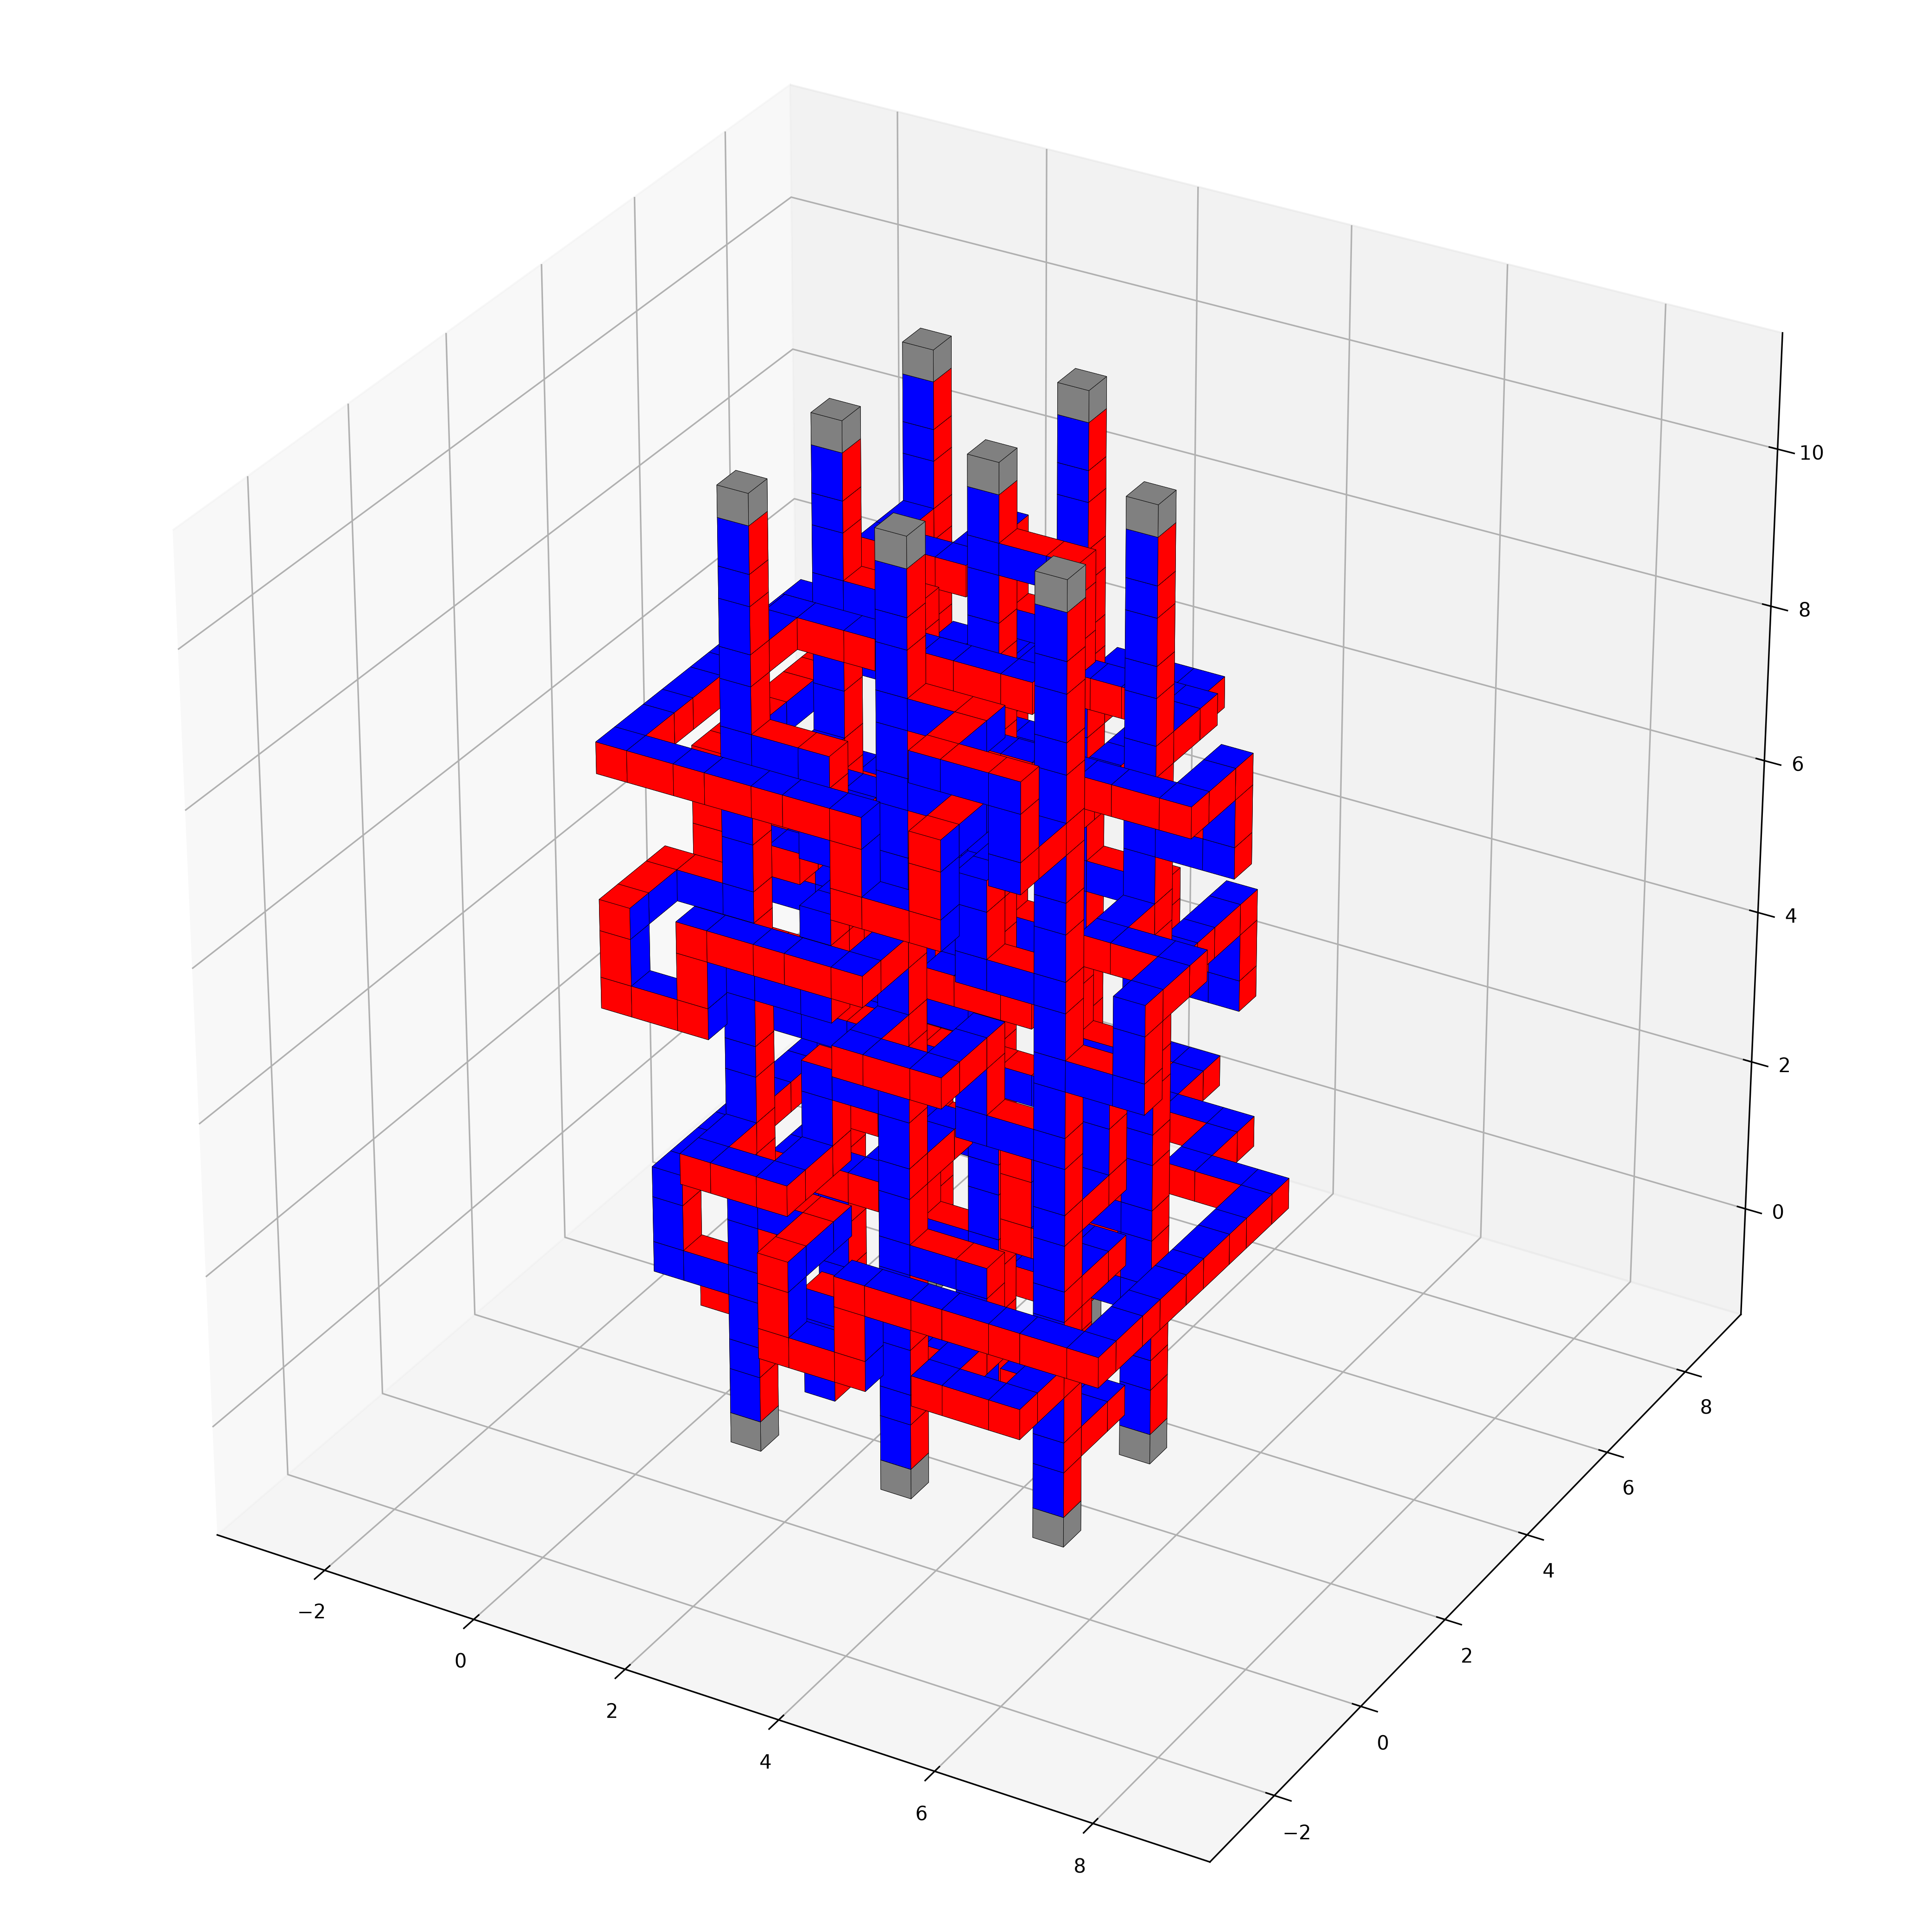
\includegraphics[width=\linewidth]{figures/ours-mqt_max_parallel.png}
        \caption{Double-slice, max-parallel.}
    \end{subfigure}
    \hfill
    \begin{subfigure}[t]{0.47\linewidth}
        \centering
        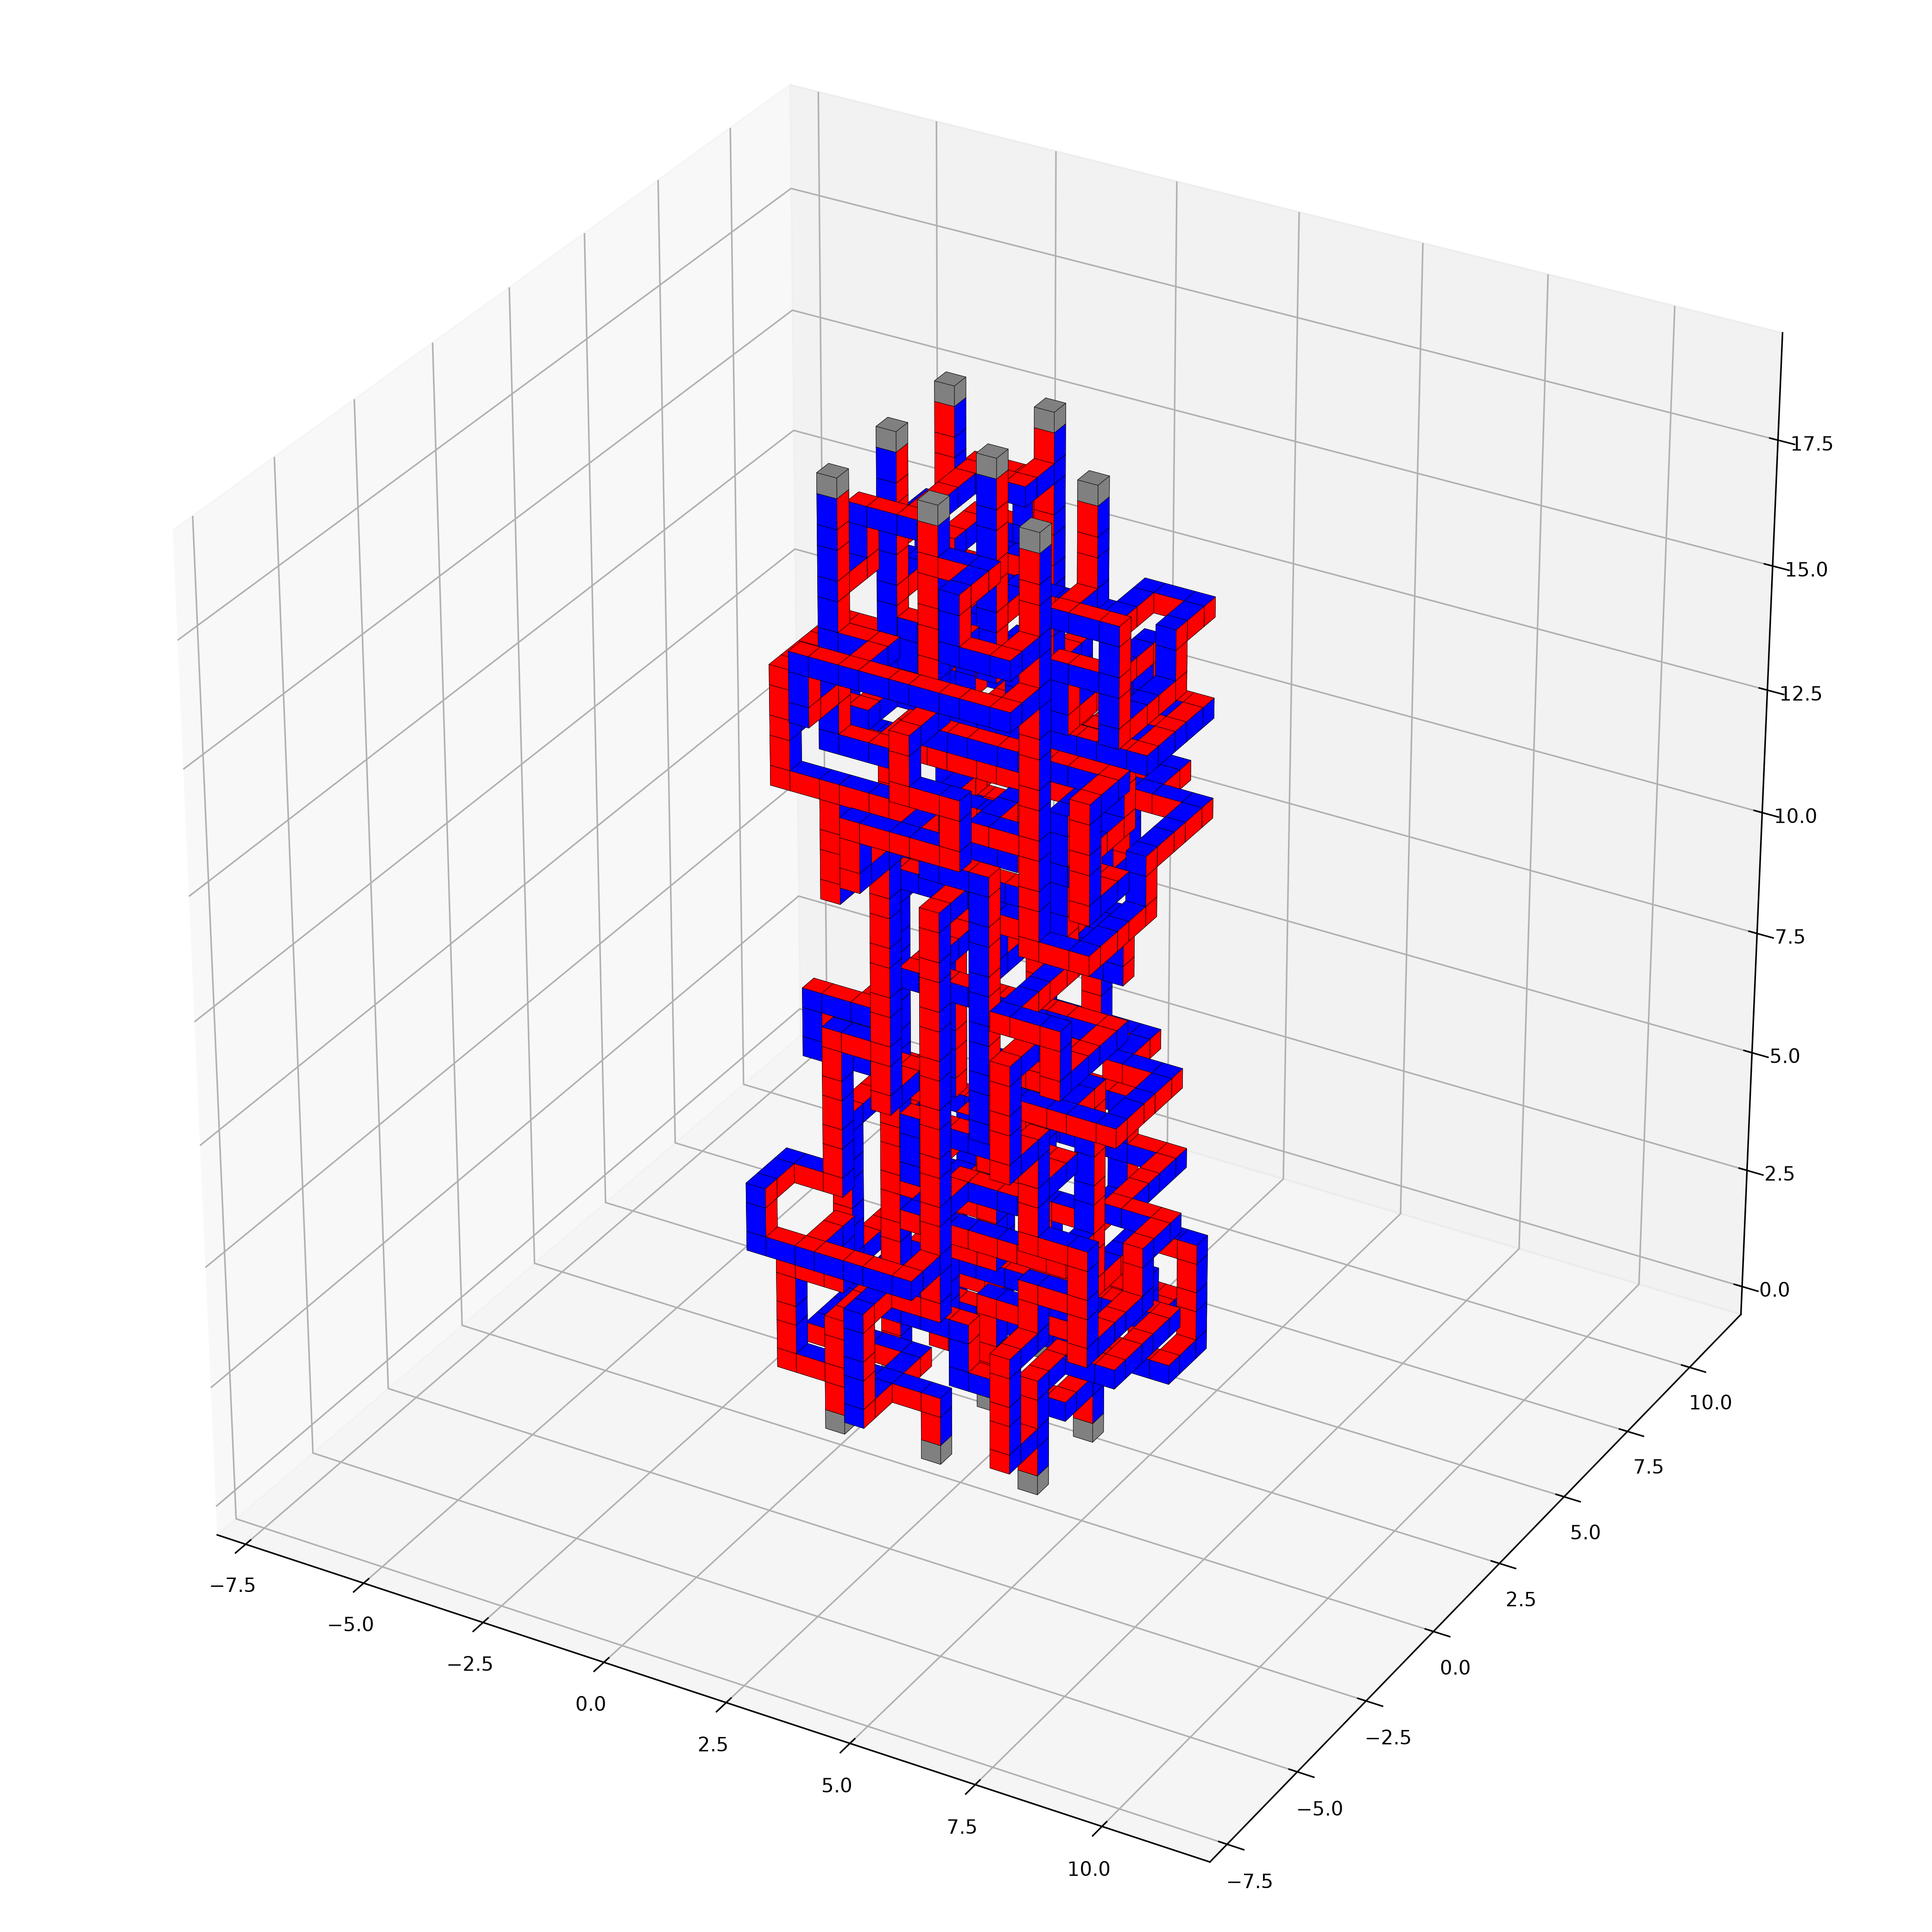
\includegraphics[width=\linewidth]{figures/topols-mqt_max_parallel.png}
        \caption{TopoLS, max-parallel.}
    \end{subfigure}
    \par\medskip
    \begin{subfigure}[t]{0.47\linewidth}
        \centering
        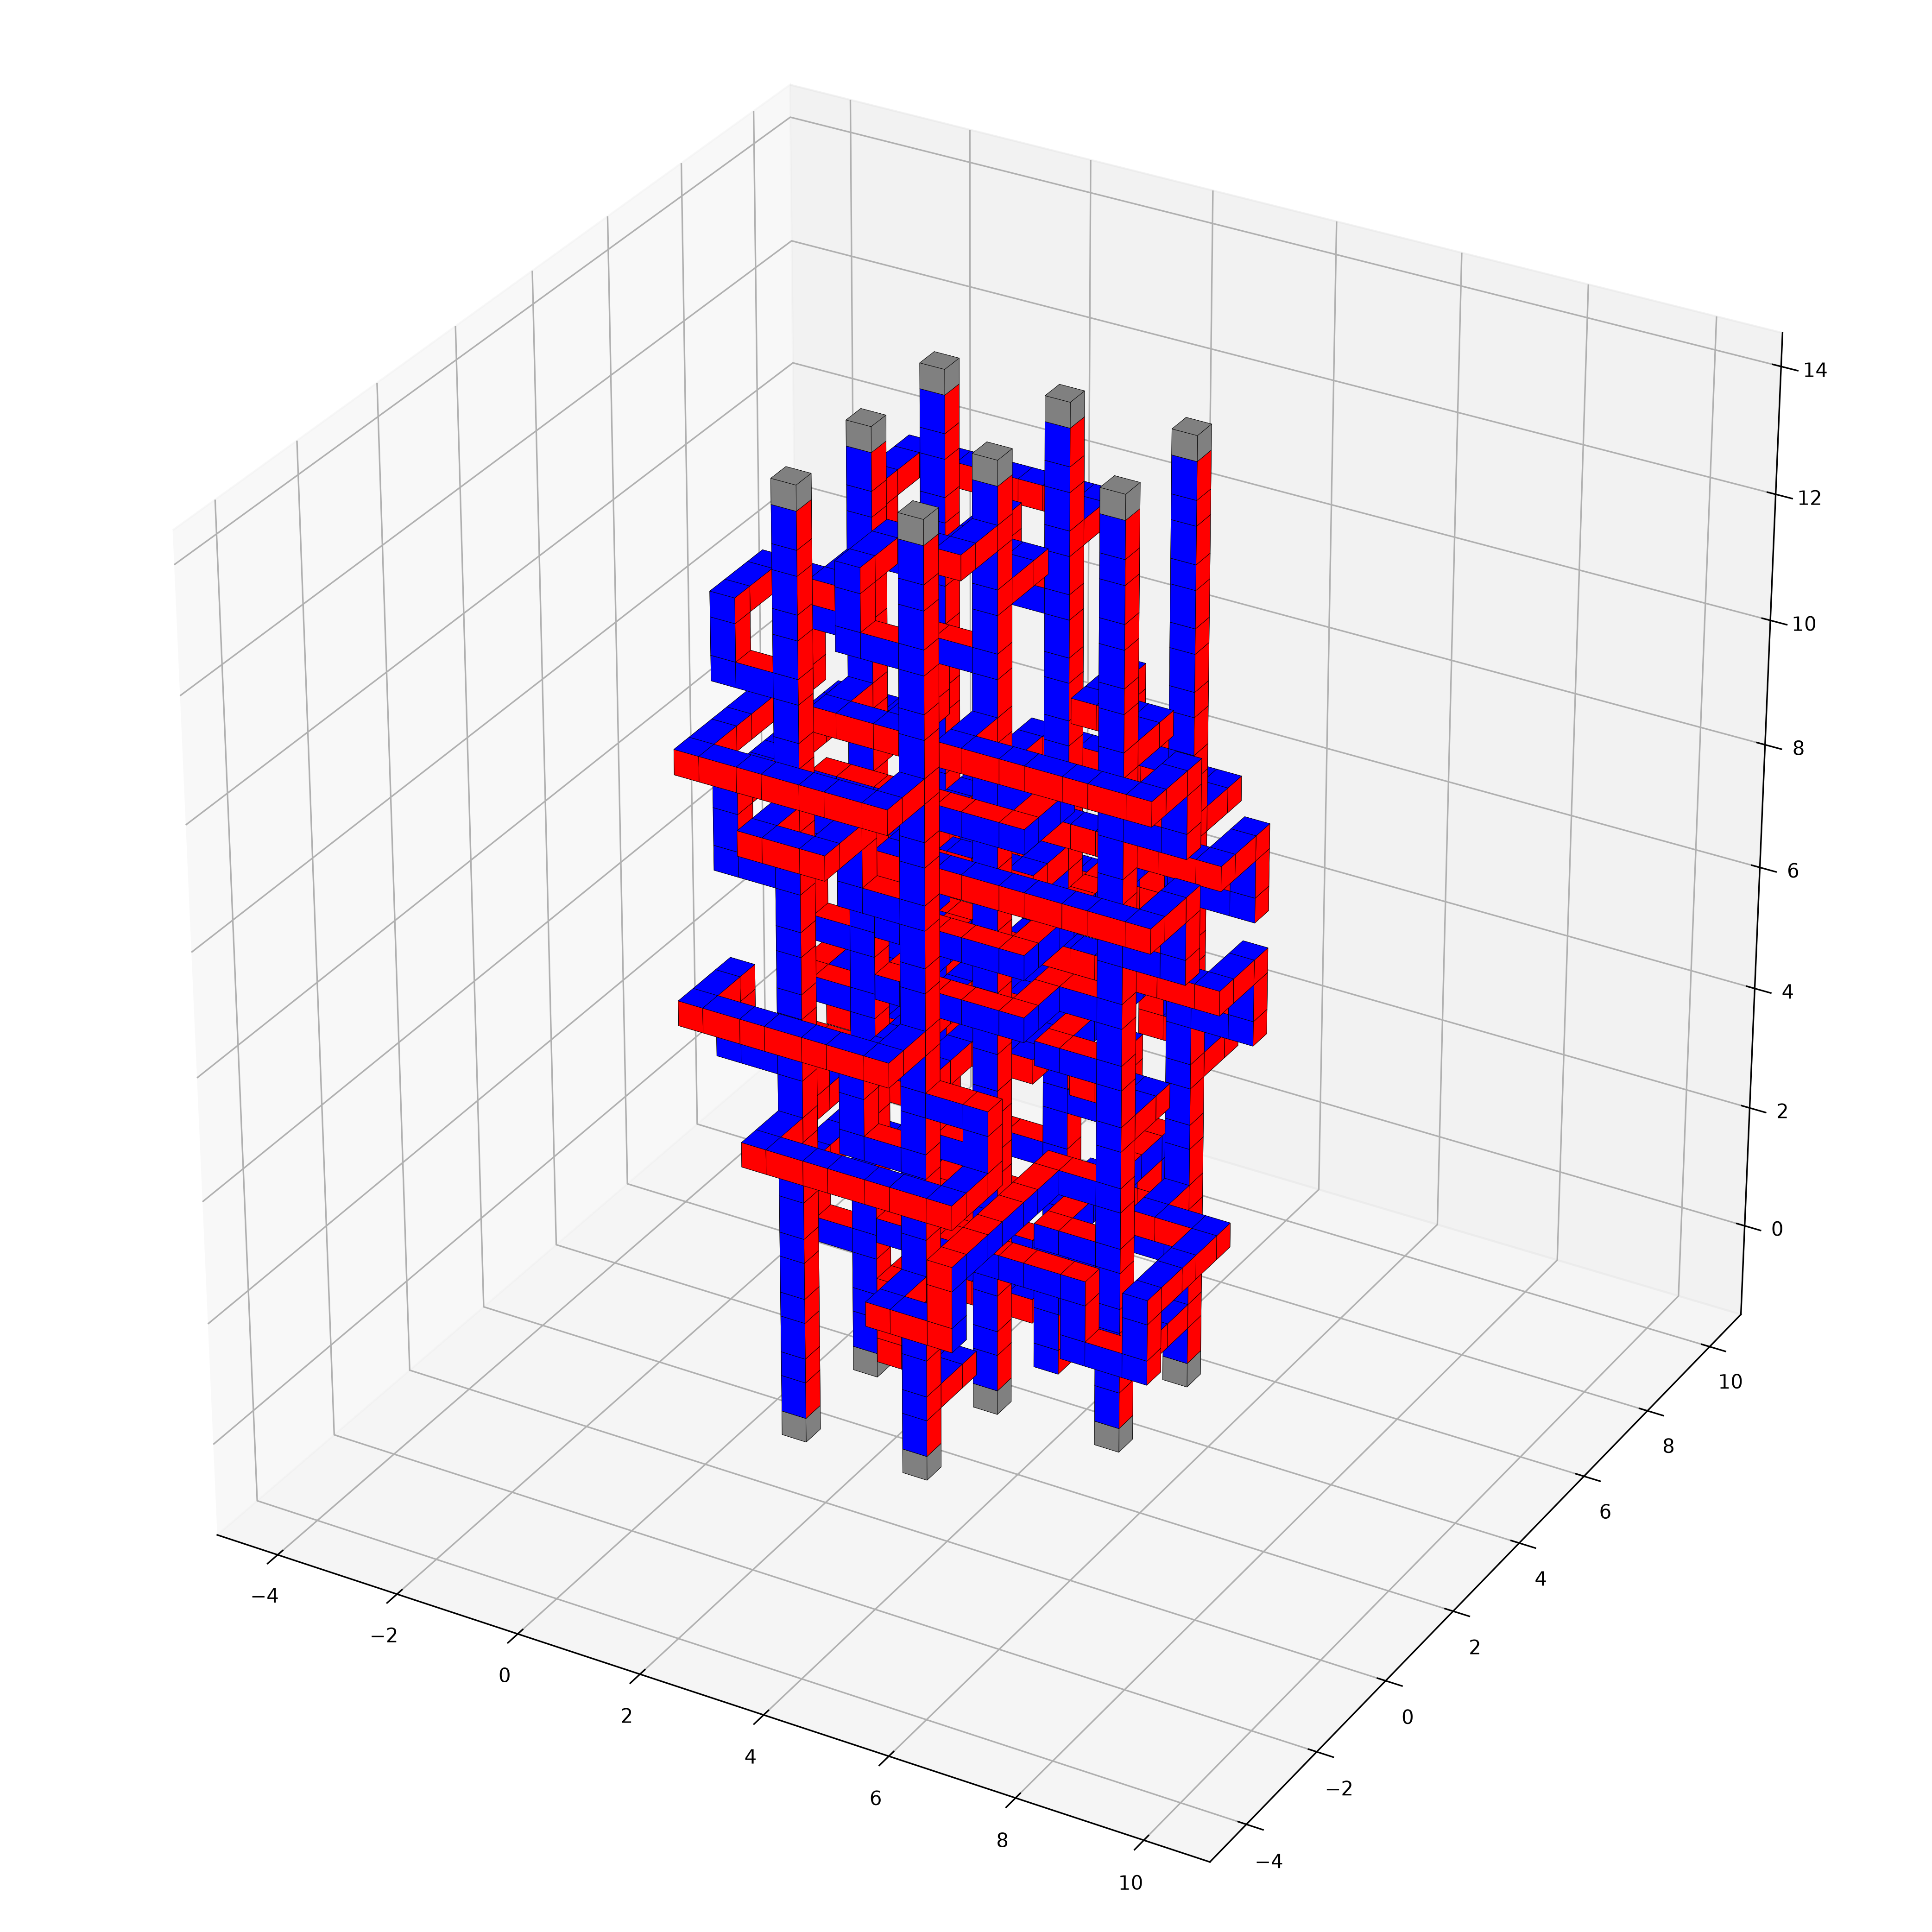
\includegraphics[width=\linewidth]{figures/ours-mqt_min_parallel.png}
        \caption{Double-slice, min-parallel.}
    \end{subfigure}
    \hfill
    \begin{subfigure}[t]{0.47\linewidth}
        \centering
        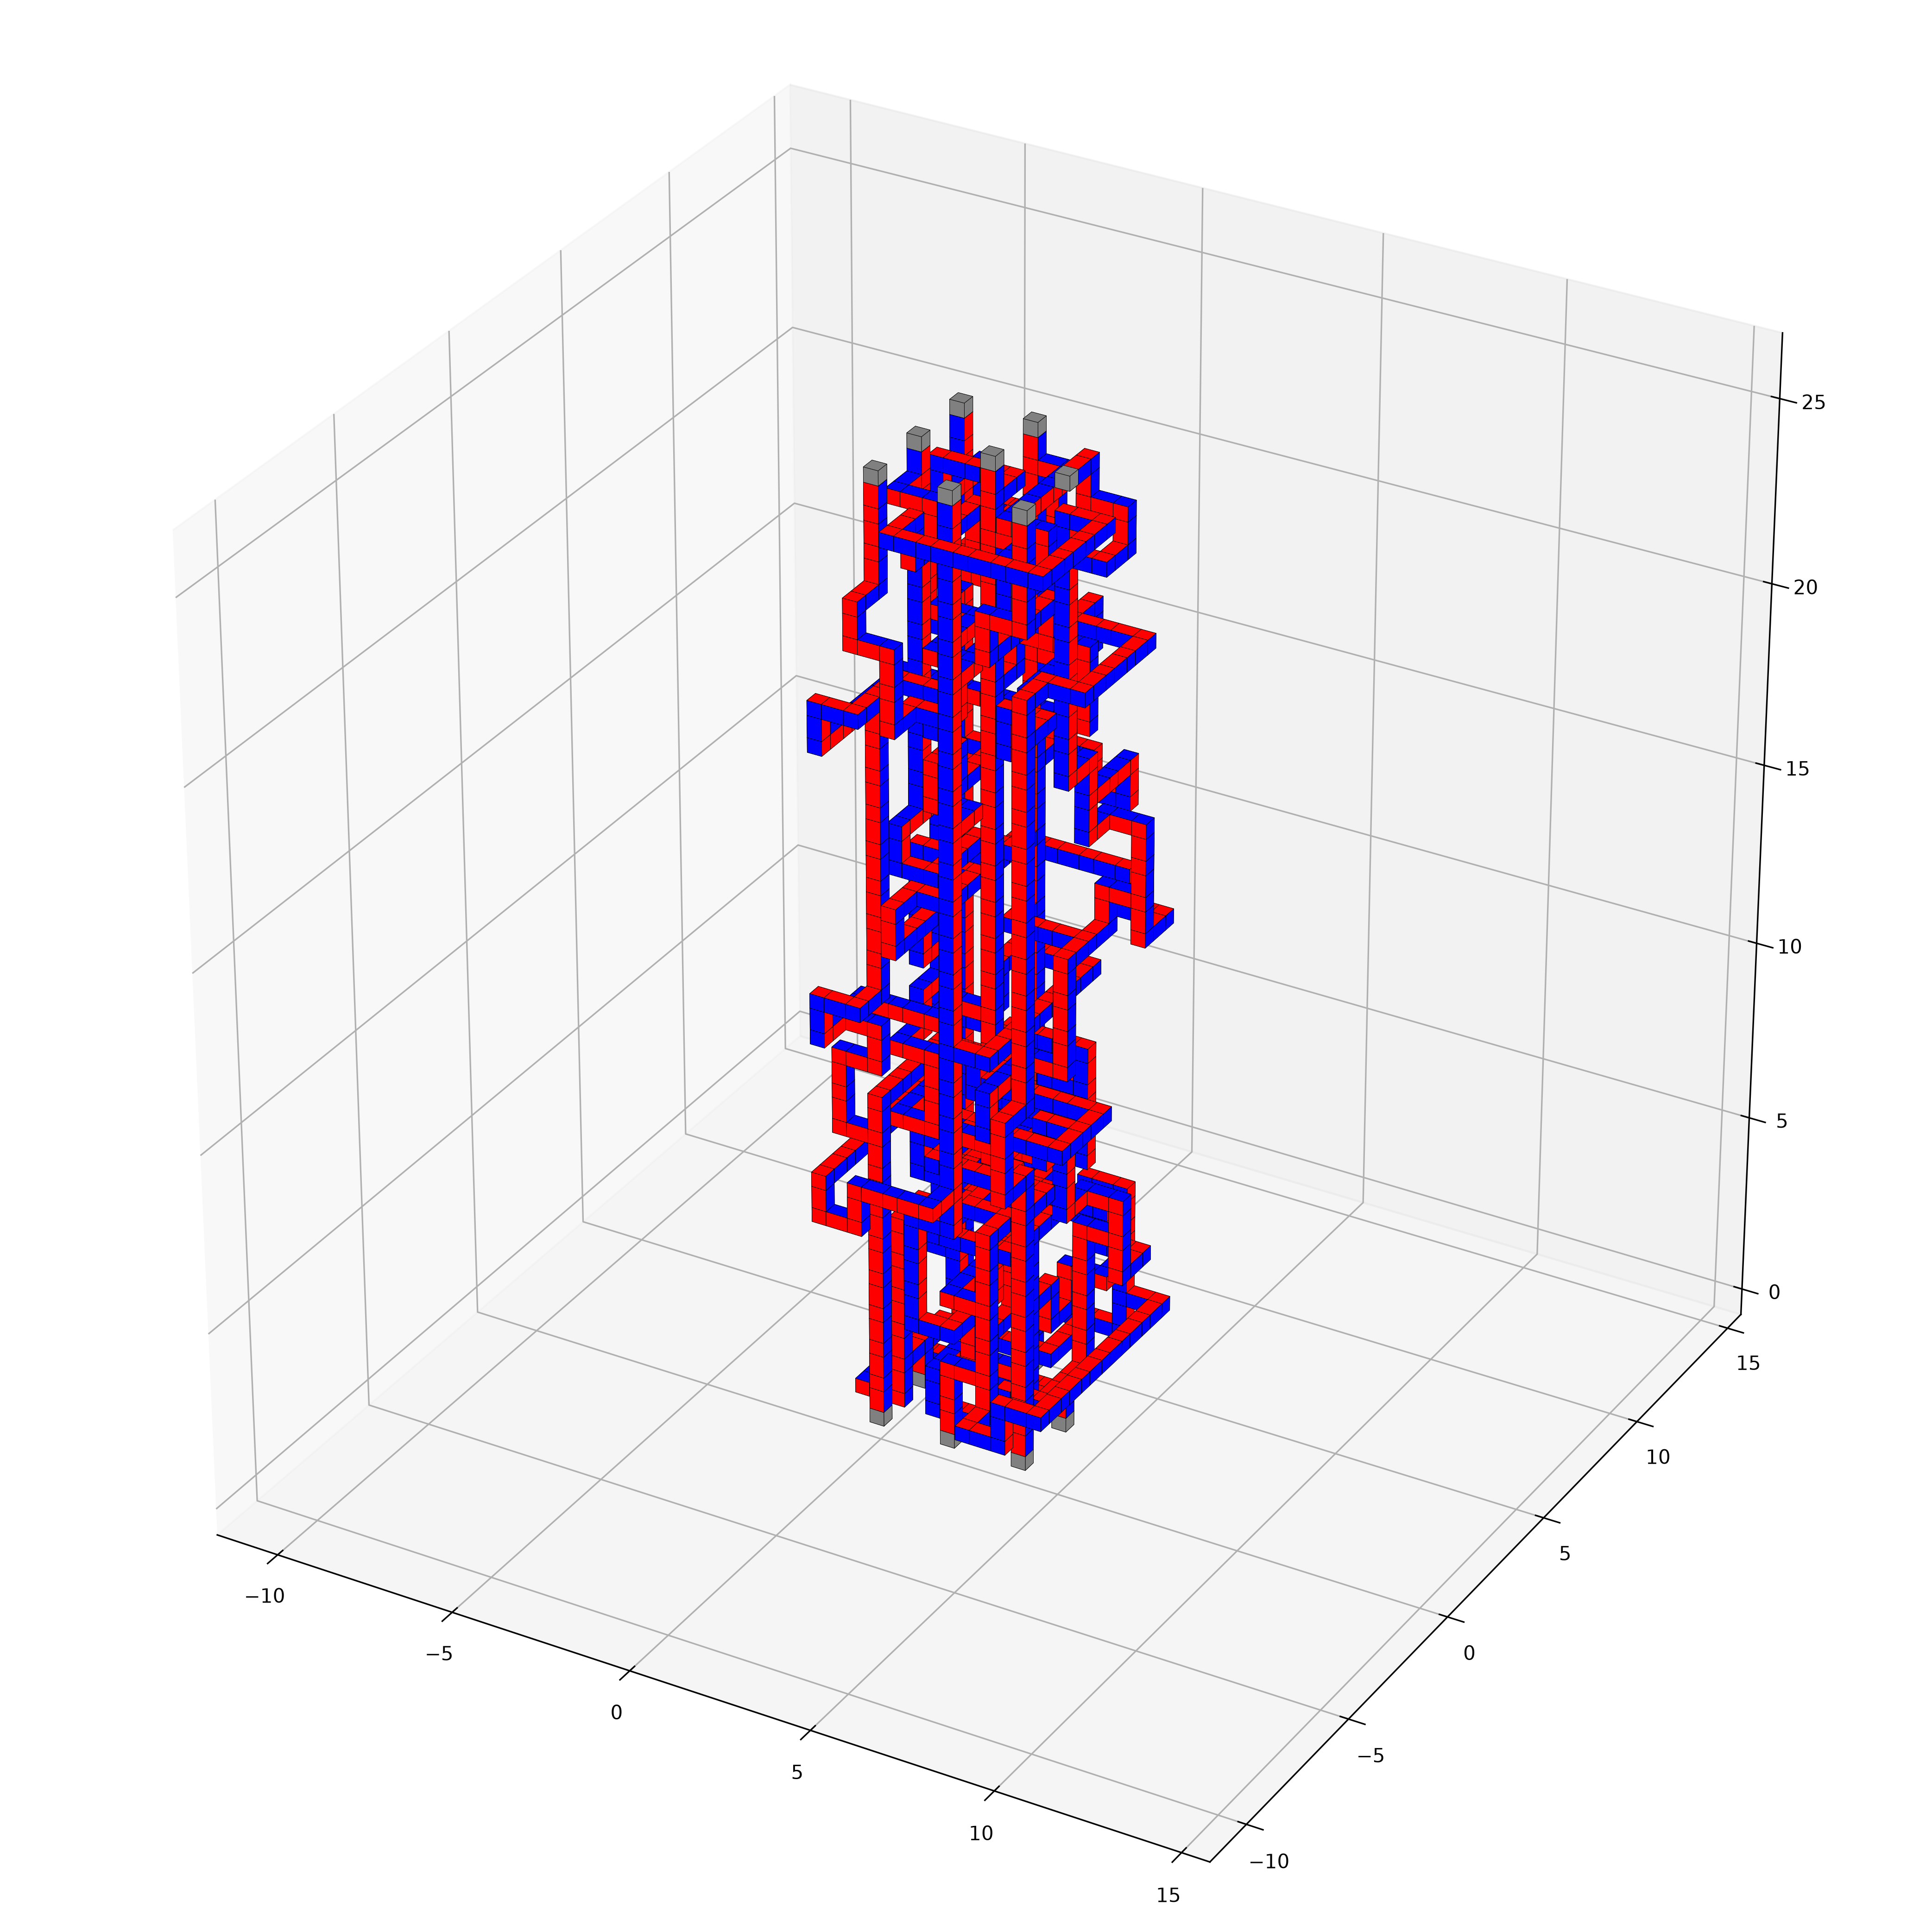
\includegraphics[width=\linewidth]{figures/topols-mqt_min_parallel.png}
        \caption{TopoLS, min-parallel.}
    \end{subfigure}
    \caption{Representative compiled spacetime geometries, rendered from TQEC BlockGraphs using TopoLS's renderer. The time direction is vertical, and blue and red faces indicate block boundary bases. Grey blocks indicate input/output ports and contribute zero volume. Each panel is independently fitted to its coordinate extent, while \cref{tab:topols_seed_sweep} provides the aggregate quantitative comparison.}
    \label{fig:comparison_embeddings}
\end{figure*}

\end{document}

